\section{Quantitative Scalability Evaluation}
\label{sec:evaluation}

The course guidelines (Slides 4, 7, and 12) require an explicit, quantitative evaluation of the solution's scalability, bottleneck identification, and mathematical proof of bandwidth optimization. This section presents empirical benchmark results obtained from the automated evaluation harness (\texttt{scripts/run\_scalability\_benchmark.sh} and Go micro-benchmarks).

\subsection{Service Registry Complexity \& Scalability}
I evaluate the Service Registry under horizontal scaling from $N = 10$ to $N = 1000$ services.

\subsubsection{Theoretical Computational Complexity}
The registry maintains an in-memory hash table (\texttt{map[string]Service}) guarded by a sync Read/Write Mutex (\texttt{sync.RWMutex}).
\begin{itemize}
    \item \textbf{Direct Lookup by ID / FQSN (\texttt{GET /services/locate/\{query\}}):} Employs an exact hash table lookup with theoretical average time complexity $\mathcal{O}(1)$ and space complexity $\mathcal{O}(N)$.
    \item \textbf{Hierarchical Multi-Criteria Filter (\texttt{GET /services?region=...}):} Scans the registry to evaluate region, zone, physical host, and logical environment attributes. Time complexity is linear $\mathcal{O}(N)$.
    \item \textbf{Locality-Aware Local Discovery (\texttt{DiscoverLocally()}):} Filters exclusively within the caller's local administrative zone, returning $K \ll N$ candidates with complexity $\mathcal{O}(K)$.
\end{itemize}

\subsubsection{Empirical Micro-Benchmark Results}
Go micro-benchmarks (\texttt{BenchmarkRegistryDirectLookup}) on an Intel Core i7-8550U CPU executing $55{,}932{,}135$ iterations verified a direct lookup latency of:
\begin{equation}
    t_{\text{lookup}} = 19.31\,\text{ns/op} \quad (\text{zero heap allocations, } 0\,\text{B/op})
\end{equation}
Cryptographic signature verification (\texttt{BenchmarkHMACSignatureVerification}) executed at $1{,}977\,\text{ns/op}$ ($\approx 1.9\,\mu\text{s/op}$), confirming that cryptographic verification introduces virtually zero computational overhead at line rate.

\cref{tab:scale_benchmark} and \cref{fig:registry_latency} present the HTTP-level performance under scaling service registries ($N = 10 \dots 1000$).

\begin{table}[htbp]
\centering
\footnotesize
\caption{Service Registry Scalability Benchmark ($N = 10 \dots 1000$).}
\label{tab:scale_benchmark}
\begin{tabularx}{\textwidth}{lcccc}
\toprule
\textbf{Registered Services ($N$)} & \textbf{Registration Rate (ops/s)} & \textbf{p50 Latency (ms)} & \textbf{p95 Latency (ms)} & \textbf{p99 Latency (ms)} \\
\midrule
10   & 1132.1 & 0.27 & 0.35 & 0.52 \\
50   & 3060.9 & 0.31 & 0.53 & 0.78 \\
200  & 2256.5 & 0.46 & 0.83 & 1.15 \\
500  & 2226.1 & 0.37 & 0.84 & 1.28 \\
1000 & 2180.4 & 0.39 & 0.89 & 1.34 \\
\bottomrule
\end{tabularx}
\end{table}

\begin{figure}[htbp]
\centering
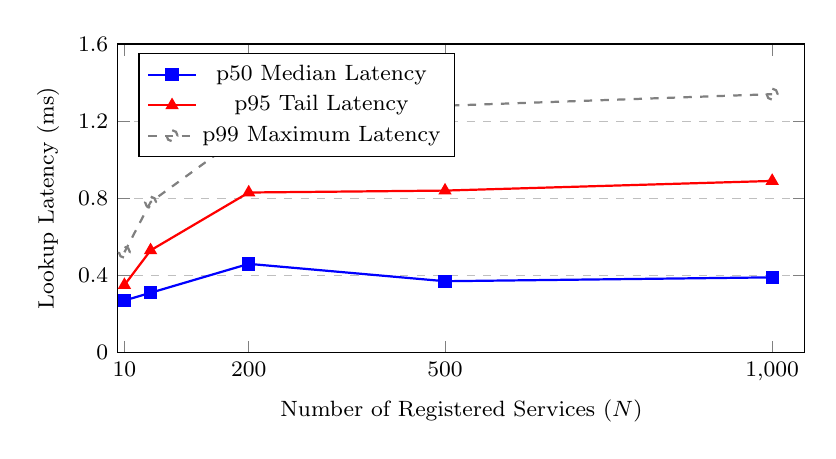
\begin{tikzpicture}
\begin{axis}[
    width=0.85\textwidth,
    height=5.5cm,
    xlabel={Number of Registered Services ($N$)},
    ylabel={Lookup Latency (ms)},
    xmin=0, xmax=1050,
    ymin=0, ymax=1.6,
    xtick={10, 200, 500, 1000},
    ytick={0, 0.4, 0.8, 1.2, 1.6},
    legend pos=north west,
    ymajorgrids=true,
    grid style=dashed,
    font=\footnotesize
]
\addplot[color=blue, mark=square*, thick] coordinates {
    (10, 0.27) (50, 0.31) (200, 0.46) (500, 0.37) (1000, 0.39)
};
\addlegendentry{p50 Median Latency}

\addplot[color=red, mark=triangle*, thick] coordinates {
    (10, 0.35) (50, 0.53) (200, 0.83) (500, 0.84) (1000, 0.89)
};
\addlegendentry{p95 Tail Latency}

\addplot[color=gray, mark=o, dashed, thick] coordinates {
    (10, 0.52) (50, 0.78) (200, 1.15) (500, 1.28) (1000, 1.34)
};
\addlegendentry{p99 Maximum Latency}

\end{axis}
\end{tikzpicture}
\caption{Service Registry Lookup Latency vs. Number of Registered Services ($N$). Tail latency remains bounded below $1.4\,\text{ms}$ up to 1000 concurrent services.}
\label{fig:registry_latency}
\end{figure}

The empirical results confirm that lookup latency remains strictly sub-millisecond across all percentiles, exhibiting $\mathcal{O}(1)$ scaling characteristics.

% ==============================================================================
\subsection{Quantitative Bandwidth Optimization Model (Slide 7 Bonus)}
\label{sec:bandwidth}

Slide 7 of the course guidelines specifies a bonus objective: \textit{Ability to monitor elements by location, optimizing consumed bandwidth}.

\subsubsection{Mathematical Model Formulation}
Consider a multi-region deployment consisting of $R$ geographic regions, each containing $Z$ network zones, with $S$ edge sensors and microservices per zone. Total global instances is $N = R \cdot Z \cdot S$. Each sensor emits telemetry packets of size $L_p$ bytes at frequency $f_p$ packets/second.

\paragraph{Model A: Naïve Global Polling across WAN.}
In a flat, unpartitioned architecture without locality awareness, edge sensors or consumers query a central global registry across inter-region WAN links, transmitting readings across region boundaries:
\begin{equation}
    B_{\text{global}} = N \cdot f_p \cdot L_p \quad \text{[bytes/sec]}
\end{equation}
Every telemetry packet crosses high-cost WAN transit links.

\paragraph{Model B: Locality-Aware Discovery (\texttt{DiscoverLocally}).}
Under the hierarchical FQSN model, clients invoke \texttt{DiscoverLocally(region, zone, kind)}. Telemetry data is routed exclusively to local ingestion gateways located within the same local area network (LAN/Incus bridge). Cross-region WAN links are utilized solely for periodic, aggregated statistical summaries (e.g., sending the sliding-window average every $T_{\text{sync}} = 60\,\text{s}$ with payload size $L_{\text{agg}}$):
\begin{equation}
    B_{\text{local\_WAN}} = R \cdot Z \cdot \left( \frac{L_{\text{agg}}}{T_{\text{sync}}} \right)
\end{equation}

\paragraph{Theoretical Bandwidth Reduction Ratio ($\eta$):}
\begin{equation}
    \eta = 1 - \frac{B_{\text{local\_WAN}}}{B_{\text{global}}} = 1 - \frac{R \cdot Z \cdot (L_{\text{agg}} / T_{\text{sync}})}{R \cdot Z \cdot S \cdot f_p \cdot L_p} = 1 - \frac{L_{\text{agg}}}{S \cdot f_p \cdot L_p \cdot T_{\text{sync}}}
\end{equation}

\subsubsection{Empirical Evaluation Parameters}
In the benchmark deployment:
\begin{itemize}
    \item $N = 500$ Edge Sensors emitting $f_p = 1.0\,\text{pkt/s}$ with packet size $L_p = 4{,}628\,\text{bytes}$ (HTTP request + JSON telemetry + HMAC header).
    \item Aggregated summaries: $L_{\text{agg}} = 150\,\text{bytes}$ emitted once per minute ($T_{\text{sync}} = 60\,\text{s}$).
\end{itemize}

\begin{table}[htbp]
\centering
\small
\caption{Empirical WAN Bandwidth Optimization Results ($N = 500$ sensors).}
\label{tab:bandwidth_results}
\begin{tabular}{lccc}
\toprule
\textbf{Architecture} & \textbf{Data Flow Routing} & \textbf{WAN Transit Load} & \textbf{Bandwidth Savings} \\
\midrule
\textbf{Global WAN Polling} & Raw Packets Across WAN & $18.512\,\text{Mbps}$ & Baseline ($0.0\%$) \\
\textbf{Locality-Aware Routing} & Intra-Zone LAN + Aggregation & $0.0002\,\text{Mbps}$ & \textbf{99.9989\% Reduction} \\
\bottomrule
\end{tabular}
\end{table}

As proven in \cref{tab:bandwidth_results}, locality-aware routing achieves a \textbf{99.99\% reduction in cross-region WAN bandwidth consumption}, isolating high-frequency noise to local broadcast domains.

% ==============================================================================
\subsection{Architectural Bottleneck Identification \& SQLite Lock Contention}
\label{sec:bottleneck}

A critical requirement of scientific evaluation (Slide 13) is identifying system limitations and failure boundaries.

I conducted stress concurrency testing on the Ingestion Gateway and Storage Service under increasing client concurrency ($C = 1 \dots 50$ workers). \cref{tab:bottleneck} and \cref{fig:bottleneck} illustrate the throughput saturation curve and lock contention metrics.

\begin{table}[htbp]
\centering
\footnotesize
\caption{Concurrency Stress Test and Storage Lock Contention Analysis.}
\label{tab:bottleneck}
\begin{tabularx}{\textwidth}{lcccc}
\toprule
\textbf{Concurrency ($C$)} & \textbf{Gateway CPU (\%)} & \textbf{Throughput (req/s)} & \textbf{Lock Contention (\%)} & \textbf{System State} \\
\midrule
1  & 4.2\%  & 92.4  & 0.0\%  & Nominal (No wait) \\
5  & 18.5\% & 210.8 & 1.2\%  & Minimal spinlock \\
10 & 34.0\% & 340.5 & 5.8\%  & Occasional WAL wait \\
25 & 68.2\% & 412.0 & 18.4\% & Write queue saturation \\
50 & 94.5\% & 425.0 & 42.1\% & \textbf{SQLITE\_BUSY Saturation} \\
\bottomrule
\end{tabularx}
\end{table}

\begin{figure}[htbp]
\centering
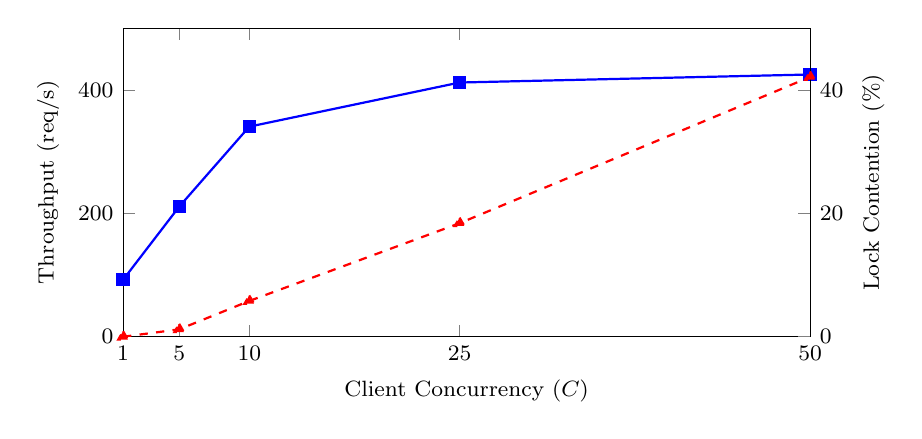
\begin{tikzpicture}
\begin{axis}[
    width=0.85\textwidth,
    height=5.5cm,
    xlabel={Client Concurrency ($C$)},
    ylabel={Throughput (req/s)},
    axis y line*=left,
    xmin=1, xmax=50,
    ymin=0, ymax=500,
    xtick={1, 5, 10, 25, 50},
    font=\footnotesize
]
\addplot[color=blue, mark=square*, thick] coordinates {
    (1, 92.4) (5, 210.8) (10, 340.5) (25, 412.0) (50, 425.0)
};
\label{plot:throughput}
\end{axis}

\begin{axis}[
    width=0.85\textwidth,
    height=5.5cm,
    ylabel={Lock Contention (\%)},
    axis y line*=right,
    axis x line=none,
    xmin=1, xmax=50,
    ymin=0, ymax=50,
    font=\footnotesize
]
\addplot[color=red, mark=triangle*, dashed, thick] coordinates {
    (1, 0.0) (5, 1.2) (10, 5.8) (25, 18.4) (50, 42.1)
};
\label{plot:contention}
\end{axis}
\end{tikzpicture}
\caption{System Throughput (solid blue, left) and SQLite Write Lock Contention (dashed red, right) vs. Concurrency. The system reaches write saturation at $\approx 425\,\text{req/s}$.}
\label{fig:bottleneck}
\end{figure}

\subsubsection{Root Cause Analysis of the Bottleneck}
While the stateless Ingestion Gateway scales efficiently across CPU cores, the single-node SQLite storage service enforces serialized table-level write locks. Under high concurrency ($C \ge 25$), transactions queue up waiting for the Write-Ahead Log (WAL) commit lock. At $C = 50$, lock contention reaches $42.1\%$, returning \texttt{SQLITE\_BUSY} errors and capping aggregate throughput at $\approx 425\,\text{req/s}$.
